\section{Introduction}
\label{sec:introduction}
% state the learning objective 
The objective of this laboratory assignment is to build a AC/DC connverter. 


% COLOCAR DADOSIn order to analyse the circuit, the following data were obtained by running the supplied Python script

\par The voltage source is defined by:
\begin{equation}
v_s(t) = V_s u(-t) + sin(2 \pi f t)u(t)
\label {equation:voltsource}
\end{equation}
, where
\begin{equation}
u(t)=
\begin{cases}
0 & $t$ < $0$ \\
1 & $t $\geq$ 0$
\end{cases}
\label {eq:ut}
\end{equation}

In Section~\ref{sec:analysis}, a theoretical analysis of the circuit, 
performed on Octave, is presented. In Section~\ref{sec:simulation}, the 
circuit is analysed by simulation, using NGSpice, and the results are compared to 
the theoretical results obtained in Section~\ref{sec:analysis}. The conclusions 
of this study are outlined in Section~\ref{sec:conclusion}.

\begin{figure}[H] \centering
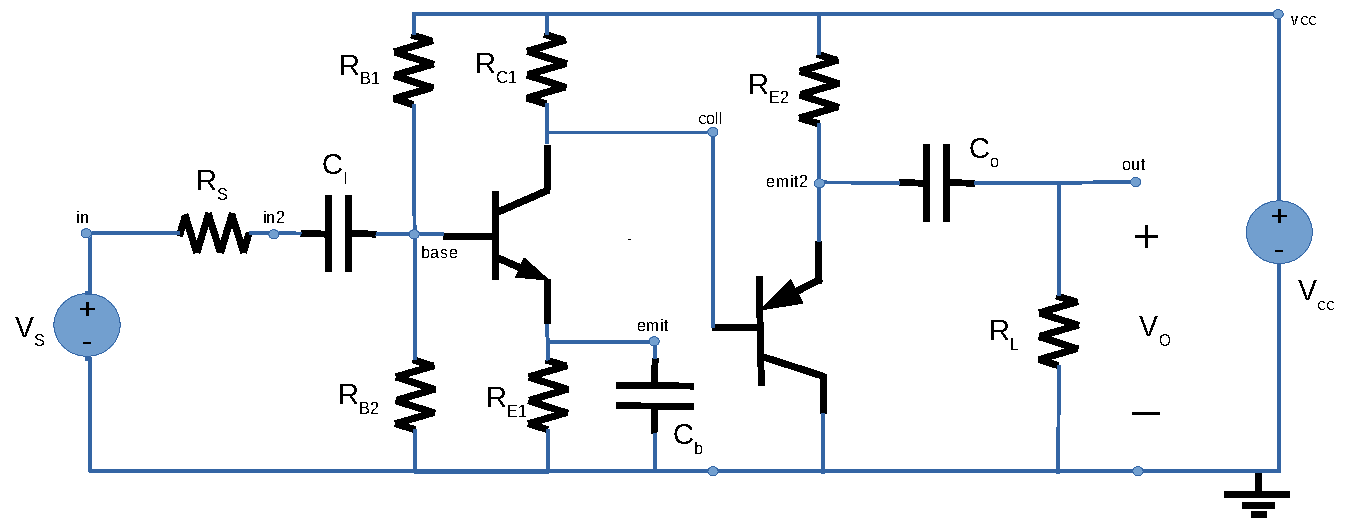
\includegraphics[width=0.4\linewidth]{circuit.pdf}
\caption{Circuit }                                     %%%%%%%%%%LEGENDA
\label{fig:circuit}
\end{figure}

